\subsection{Maximierung des Zuwachses der Erkennungsgenauigkeit}
Standardmäßig wächst ein Entscheidungsbaum solange es mindestens eine Teilung gibt, die die Erkennungsgenauigkeit erhöht. Das führt zu sehr großen und sehr granularen Entscheidungsbäumen, die die Trainingsmenge
auswendig lernen. Zudem sind die Bäume meistens unbalanciert es gibt viele Teilungen, die die Erkennungsgenauigkeit nur sehr geringfügig erhöhen.
\newline
\newline
Scikit-Learn bietet eine Reihe an Hyperparametern um dieses Verhalten zu steuern. Eine vollständige Analyse aller Parameter würde den Rahmen dieser Arbeit sprengen. Aus diesem Grund wird sich auf
den Parameter \texttt{min\_samples\_leaf} beschränkt. Es wird immer eine feste Maximalhöhe von 16 betrachtet und mit der Optimierungsstufe \textit{Os} kompeliert.
\newline
\newline
\subfigbox{
\subfigure[Trainingsmengengröße: 1023]{\label{subfig:msl_small}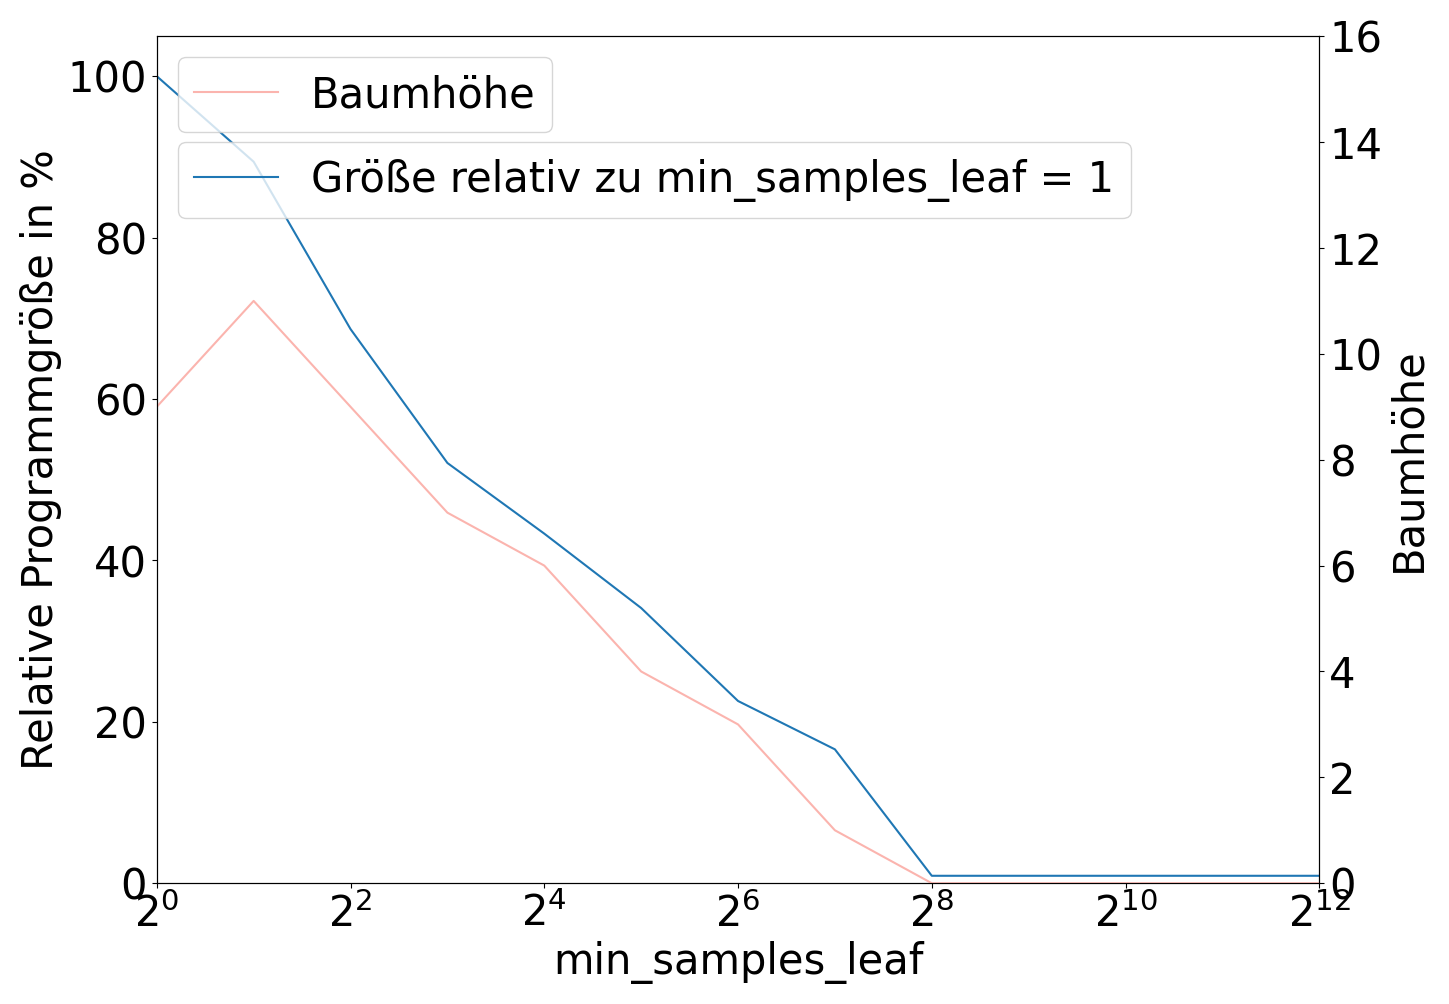
\includegraphics[width=0.48\linewidth]{images/min_samples_leaf_small.png}}\hfill%
\subfigure[Trainingsmengengröße: 7629]{\label{subfig:msl_big}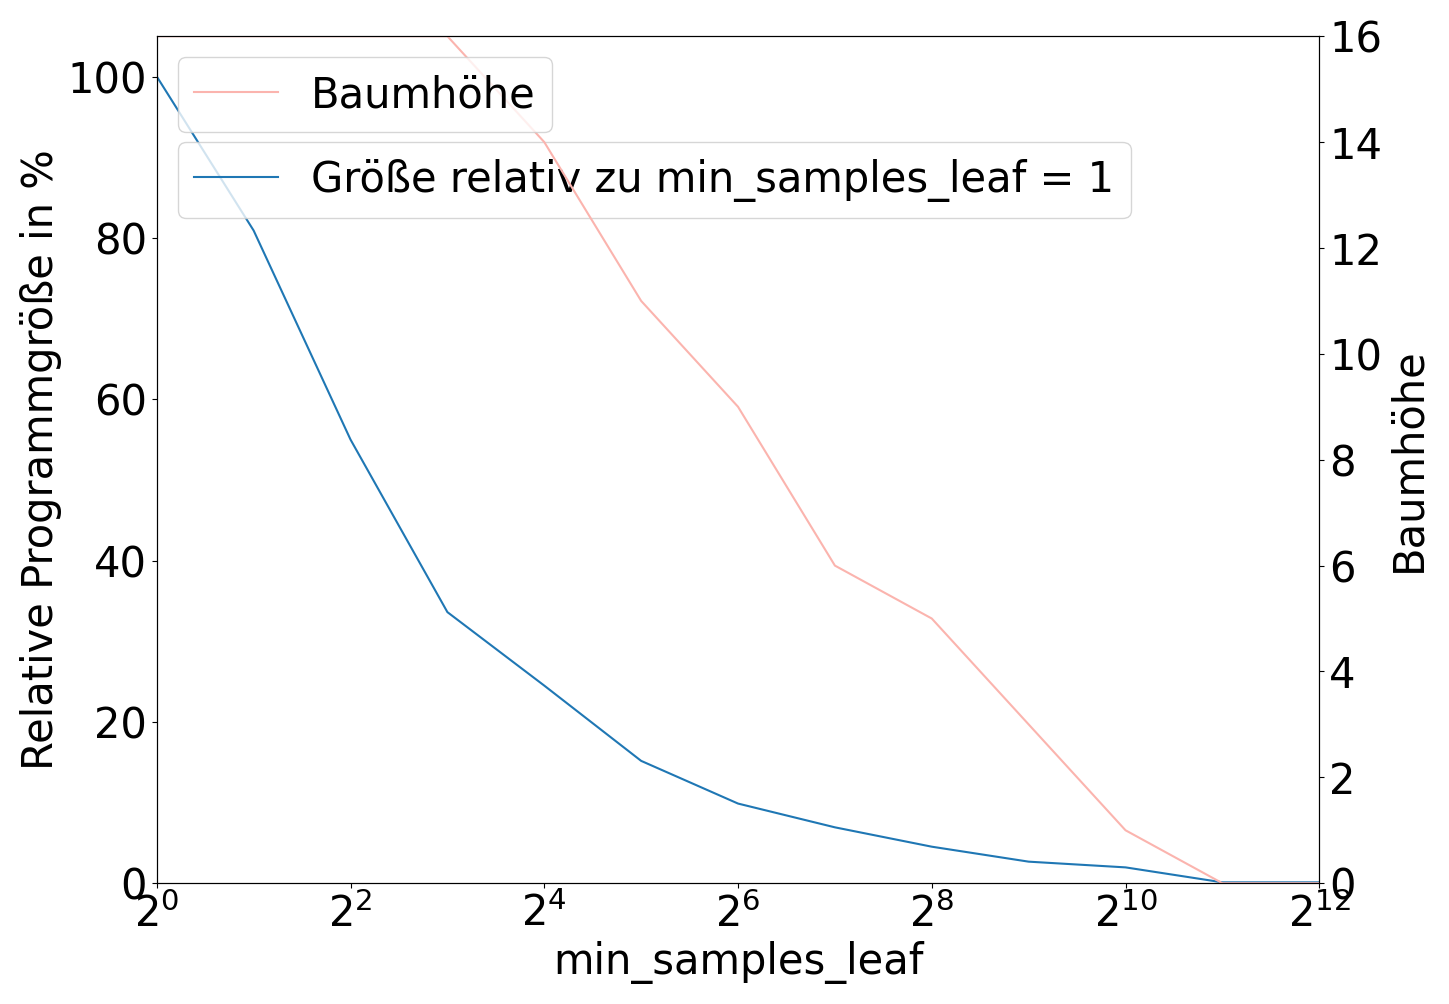
\includegraphics[width=0.48\linewidth]{images/min_samples_leaf_big.png}}%
}{Auswirkung von \texttt{min\_samples\_leaf} Parameter auf resultierende Programmgröße und Baumhöhe.}{fig:msl}
Damit eine Teilung stattfinden kann, muss der Knoten mindestens \texttt{min\_samples\_leaf} Einträge enthalten. Standardmäßig ist der Wert 1
\cite{ScikitLearnDTC}. Abbildung \ref{fig:msl} zeigt die relative Programmgröße zu der Konfiguration mit $\texttt{min\_samples\_leaf}=1$ und die resultierende maximale Baumhöhe die erreicht wurde.
Zu sehen ist, dass bereits kleine Werte die Programmgröße signifikant verringern. Dieser Effekt ist größer bei großen Trainingsmengen und kleiner bei kleinen Trainingsmengen. Gleichzeitig verringert
sich aber auch die maximale Baumhöhe die erreicht wird. Bei der großen Trainingsmenge hat sich die Programmgröße um $66,6\%$ verringert bei gleichbleibender Baumhöhe mit $\texttt{min\_samples\_leaf}=16$.
\texttt{min\_samples\_leaf} eignet sich dementsprechend am besten für große Trainingsmengen.